\subsection{Inner Loop}
In this section the inner loop controller is designed. The inner loop has the purpose of controlling the motors and wheels model and ensure that the effect of noise and uncertainties in the system are diminished, resulting in better performance for the balancing segway.\newpage
The transfer function for the motors and wheels is:
%that the input for the outer loop, the inverted pendulum model, is 1, as this will eliminate noise and ensure a more efficient cascade controller. This will result in a more stable balancing segway. The motors and wheels model is the following expression.
\begin{equation}
G_2(s)=\frac{17.72}{s+9.799} = \frac{1.81}{0.10s + 1}
\end{equation}
\begin{where}
\va{$G_2(s)$}{is the plant of the inner loop}{1}
\end{where}

The motors and wheels model is a first order system with a pole in -9.799. This means it is a type 0 system, as it does not have any poles in zero. This reveals some characteristics of the system. One of these is the presence of a steady-state error in its step response \citep[p. 211]{sou:Feedback}. This can only be fully eliminated if an integrator is implemented, as this yields a type 1 system. It is however chosen not to do this, but instead only implement a gain as this is assumed to reduce the steady-state error adequately and allows for a simpler controller design. A P-controller is therefore designed for the inner loop. A P-controller has the form as seen below:
\begin{equation}
D_2(s)=k_{p2}
\end{equation}
\begin{where}
\va{$D_2(s)$}{is the controller for the inner loop}{1}\\
\va{$k_{p2}$}{is the proportional gain}{1}
\end{where}

To design a P-controller it is necessary to look into how fast the system is sampled as this, together with saturation, sets an upper limitation for how much gain the system can handle. However, in the design of this controller, the saturation is disregarded as it is assumed that the influence is negligible. The motors' encoders sample with a frequency of 1 kHz. This is also the frequency of the inner loop. It is preferable, by rule of thumb, to have a system bandwidth that is more than 25 times smaller than the angular sampling frequency \citep[p. 613]{sou:Feedback}. It is however chosen to design with a factor of 10. Note that the sampling frequency is converted from hertz to radians per seconds, and thus the bandwidth is found as:

\begin{equation}
\omega_{BW} = 2\pi\cdot \frac{f_s}{10}= 2\pi\cdot\frac{1000}{10}= 628.32 \label{eq:motorbandwidth}
\end{equation}
\begin{where}
\va{$\omega_{BW}$}{is the bandwidth of the inner loop}{rad/s}
\va{$f_s$}{is the sampling frequency of the inner loop}{Hz}
\end{where}

From \autoref{eq:motorbandwidth} the bandwidth of the plant in the inner loop is found to be 628.32 rad/s. By examining the bode plots of the plant without a controller, the plant's gain can be determined.\vspace{-1 cm}
\begin{figure}[H]
\centering
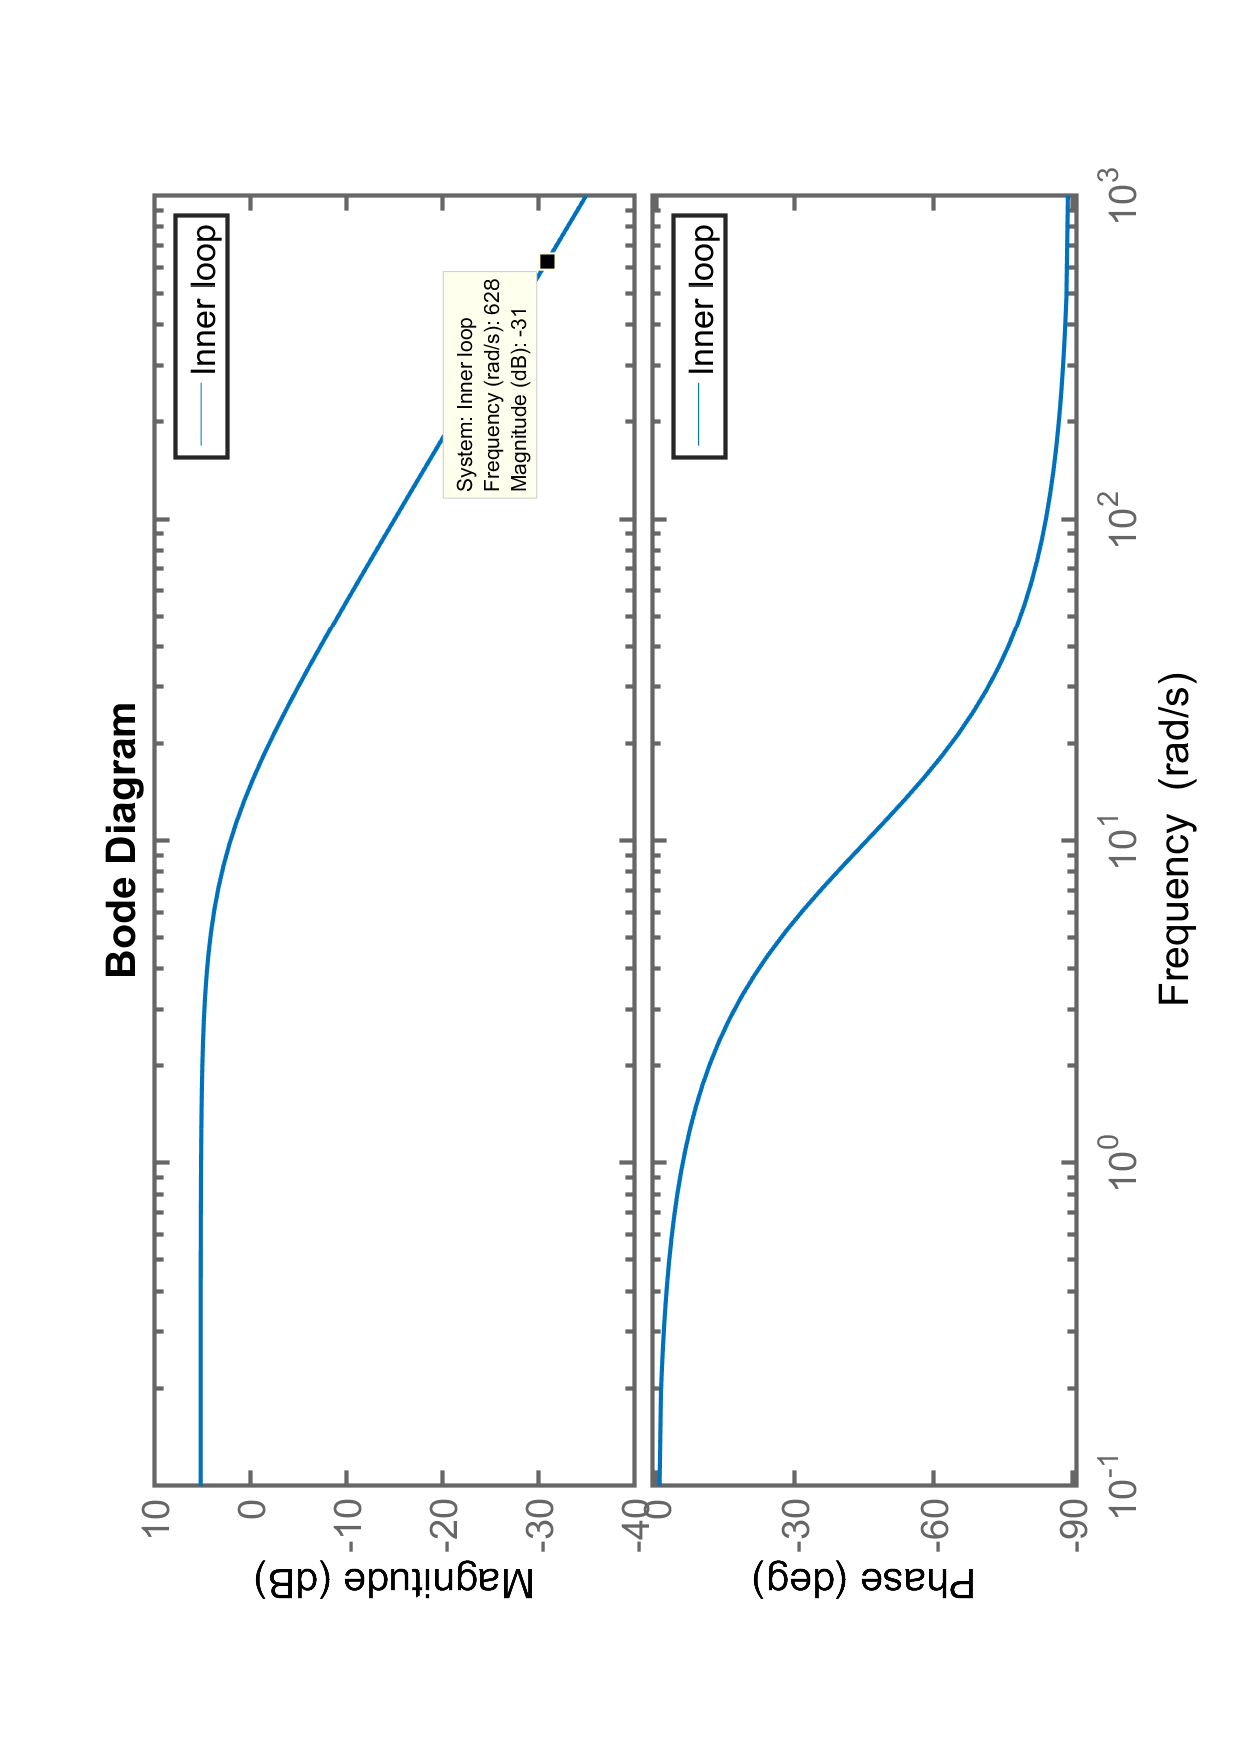
\includegraphics[height = \textwidth, angle = -90]{bodemotorplant.pdf}
\caption{Open loop bode plots of motors and wheels model, where the controller has a gain of 1. The approximate bandwidth, 628 rad/s, is marked.}
\label{fig:bodemotorplant}
\end{figure}
\vspace{-0.7 cm}
From \autoref{fig:bodemotorplant} it can be seen that the magnitude is approximately -31 dB. To obtain a magnitude of -3 dB, the graph shall be lifted 28 dB. The scalar gain can be found as follows:
\begin{equation}
k_{p2}=10^\frac{28}{20}= 25.11 \label{eq:dbscalar}
\end{equation}
The P-controller has now been designed and will in the following section be verified.
\subsection{Verification of Inner Loop Controller}
The gain for the inner loop controller shall be 25.11 according to \autoref{eq:dbscalar}. The transfer function of the closed loop can be expressed as shown in \autoref{eq:clmotor} where $H_2(s)$ is 1, due to no gain in the sensor block.
\begin{align}
\frac{Y_2(s)}{R_2(s)}=\frac{D_2(s)\cdot G_2(s)}{1+D_2(s)\cdot G_2(s)\cdot H_2(s)}
= \frac{25.11\frac{17.72}{s+9.799}}{1+25.11\frac{17.72}{s+9.799}} \label{eq:clmotor}
\end{align}
\begin{where}
\va{$Y_2(s)$}{is the output of the inner loop}{1}\\
\va{$R_2(s)$}{is the reference to the inner loop}{1}\\
\va{$H_2(s)$}{is the sensor block in the inner loop}{1}
\end{where}

\begin{figure}[H]
\centering
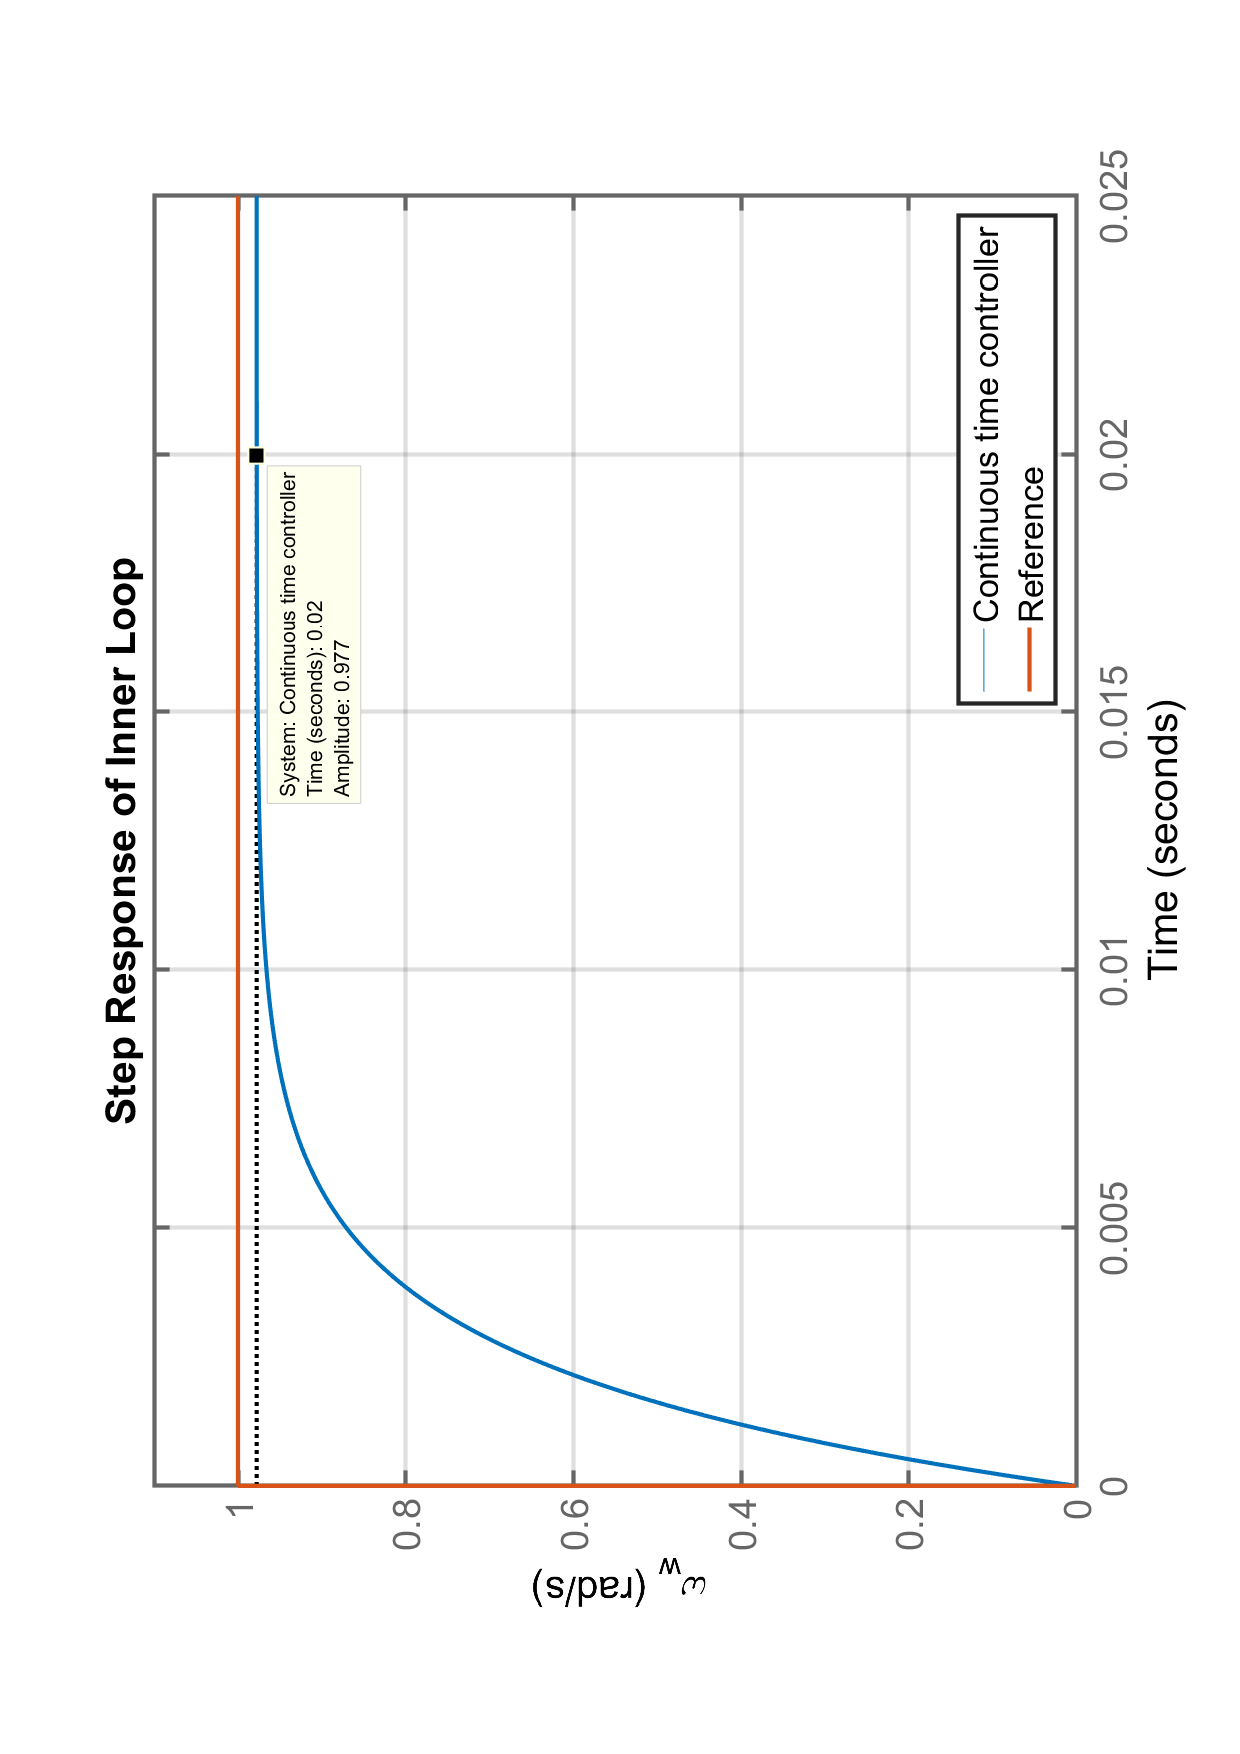
\includegraphics[height = \textwidth, angle = -90]{stepmotor25.pdf}
\caption{Simulation of the step response for inner loop with the designed continuous time P-controller.}
\label{fig:stepmotorcontroller}
\end{figure}

From \autoref{fig:stepmotorcontroller} it can be seen, that the steady-state error is 2.2\% which is deemed small enough that effect of this error on the full segway system is negligible. When looking at the characteristic equation, which is the main denominator in the closed loop transfer function, it can be seen that the gain changes the pole placement. The pole is moved far out in the left half plane (LHP). This increases the speed of the inner loop's dynamics, which can be seen in \autoref{fig:stepmotorcontroller}, where the step response settles within 0.02 seconds. 
%This results in the outer loop's input being 1, which is desired.\\ 

The closed loop transfer function is now discretized using MATLAB. The method used is the bilinear transformation, which is further described in \autoref{sec:bilinear}. This yields:
\begin{equation}
\frac{Y_2(z)}{R_2(z)} = \frac{0.2151 z^2 + 0.002119 z - 0.213}{ 1.215 z^2 - 1.978 z + 0.7674}
\end{equation}

This is compared to the continuous time controller which can be seen in \autoref{fig:sysStep1}. 

\begin{figure}[H]
\centering
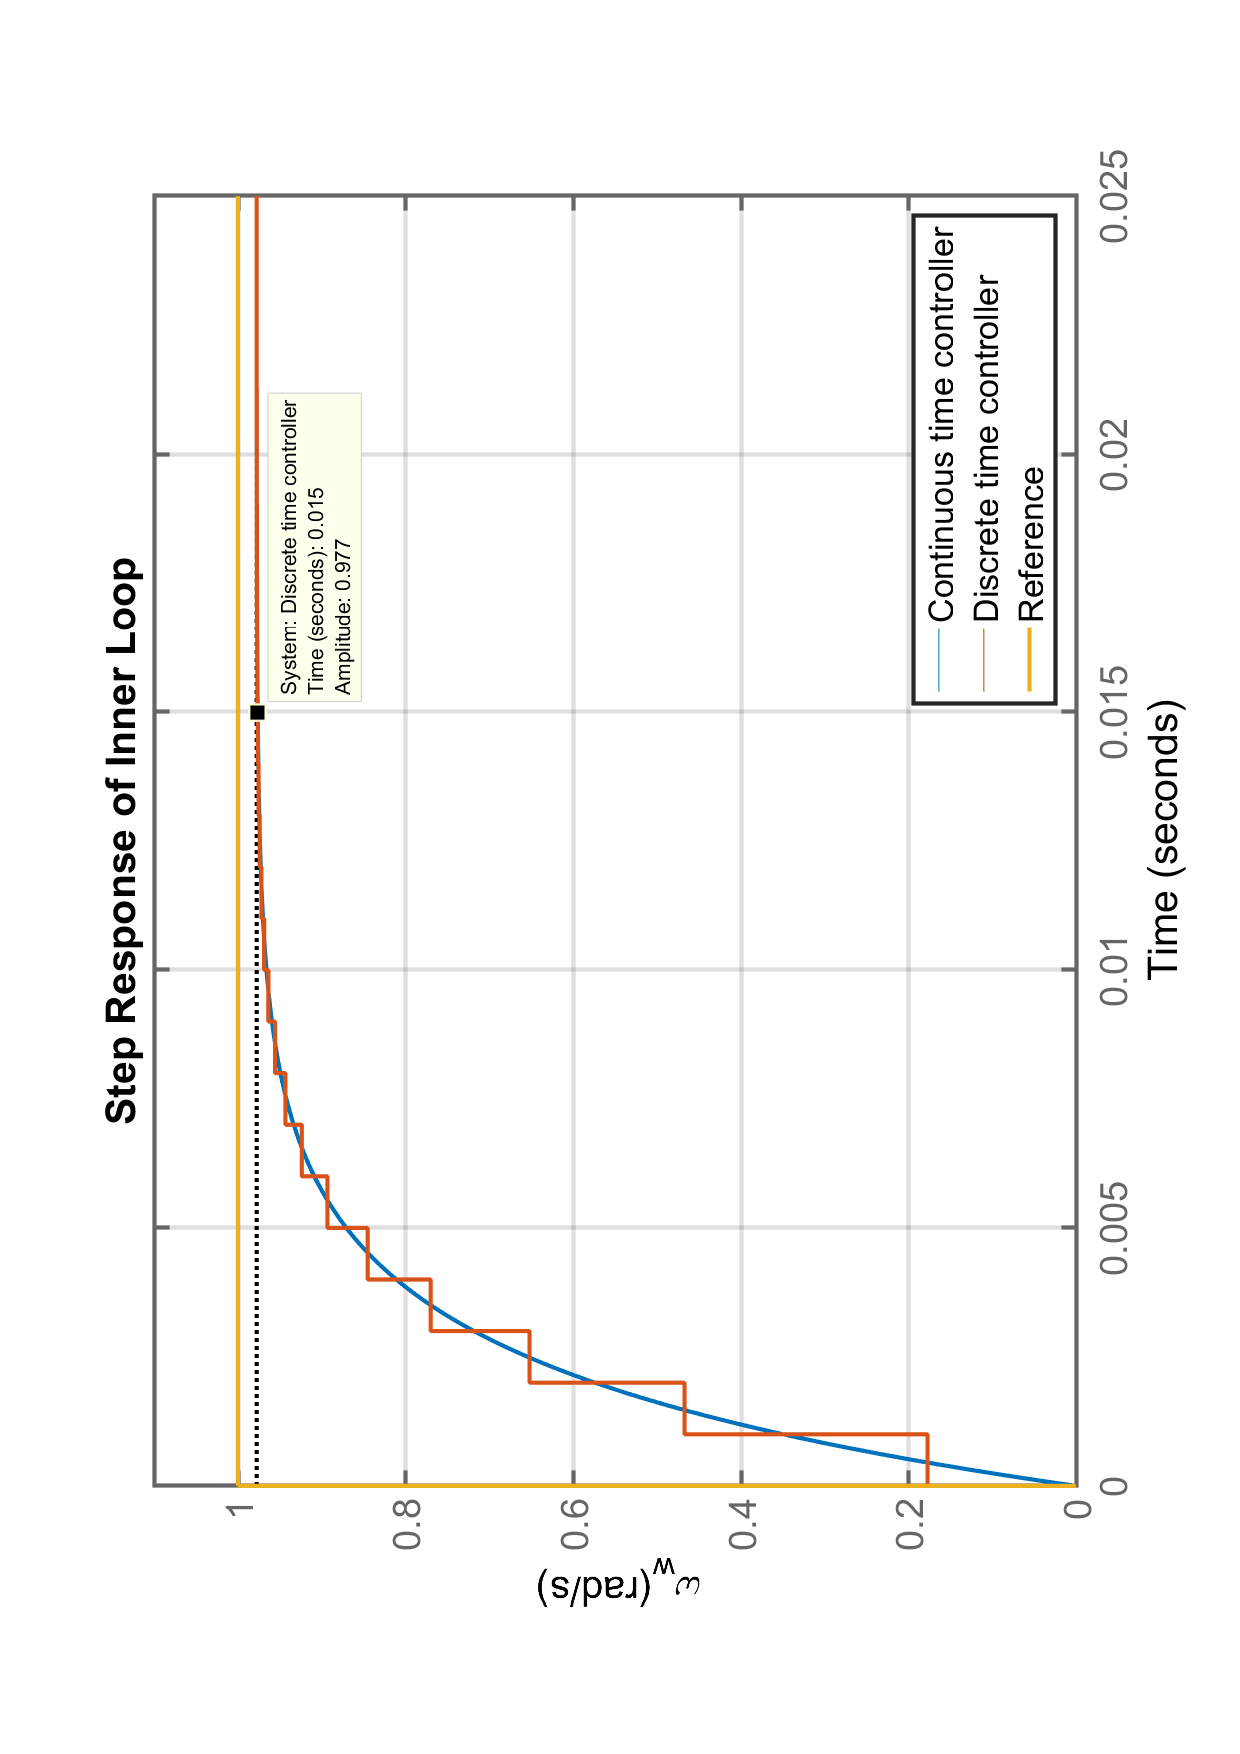
\includegraphics[height =\textwidth ,angle = -90]{sysStep1.pdf}
\caption{Simulation of the step response of continuous and discrete time inner loop controller.}
\label{fig:sysStep1}
\end{figure}

From \autoref{fig:sysStep1} it can be seen that the discrete controller matches the continuous controller and the P-controller with a gain of 25.11 for the inner loop is hereby derived. It can further be seen, that at 15 ms the velocity has almost reached its steady-state value, which means that if 15 ms is chosen as sampling time for the outer loop, the inner loop can be seen as 1 in this regard.

The outer loop will be designed in the following section. These two loops forms the cascade controller for the full system.